\documentclass[UTF8]{article}
\usepackage{ctex}
\usepackage{amsmath}
\usepackage{graphicx}

\begin{document}
\section{机械波}
\subsection{机械波的基本属性}

    一、波的定义:波是自然界中一种常见的物质运动形式,波仅伴随着加载信息的能量传递

    质点运动:实体载着信息和能量运动,若干包含能量的小的物质集合的整体运动

    波的传播:信息和能量的传播,没有物质实体的移动,能量的扩展分布,充满其传播空间

    二、波的分类:

    1.机械波:机械振动在弹性介质中的传播,在介质中传播时受牛顿定律的支配

    2.电磁波:可以在真空中传播

    3.物质波:微观粒子具有波动性,反应概率密度的空间分布

    波的共同属性:都伴随能量传播,有反射、折射、干涉、衍射现象

    三、机械波的基本属性:机械振动(波源)在弹性介质(通过相互之间的弹性力组合在一起的连续介质)中的传播形成机械波。
    
    机械波产生条件:振源+弹性介质

    是运动状态的传播,弹性介质的质点并不随波传播.
    
    四、横波和纵波

    1.横波:质点振动方向与波的传播方向相垂直的波。特征:具有交替出现的波峰和波谷;仅在固体中传播

    2.纵波:质点振动方向与波的传播方向相平行的波。固、液、气体中均可传播

    横波和纵波都是行波

\subsection{机械波的描述}

    一、波线和波面

    波面:某时刻,同一波源向外传播的波到达的空间各点连成的面(同相位面)
    
    波阵面:波在传播过程中行进在最前面的波面,又称波前

    波(射)线:描述波传播的方向的射线。在各向均匀介质中波射线垂直于波面,波射线是波的能量传播方向

    根据波面的形状,可以将波分为:球面波(点源)、柱面波(线源)、平面波(面源)

    二、波函数与波动曲线

    波形图:$y = y(x,t)$,某时刻各点振动的位移y(广义:任一物理量)与相应的平衡位置坐标x的关系曲线

    三、机械波的特征量

    振幅:A\;\;质点偏离自身平衡位置所达到的最大正向位移

    波长:$\lambda$\;\;一个完整波形的长度。即:沿波的传播方向,两个相邻的、相位差为$2\pi$的振动质点之间的距离

    周期:T\;\;波前进一个波长的距离所需要的时间

    频率:单位时间内波动所传播的完整波的数目,$\nu = \frac{1}{T}$

    周期或频率只决定于波源的振动

    波速:u\;\;波动过程中,某一振动状态(即振动相位)单位时间内所传播的距离(相速)

    \[u = \frac{\lambda}{T} = \lambda\nu]\;\;\;\lambda = \frac{u}{\nu} = Tu\]

    波速只决定于媒质的性质

    固体内:横波\;$u = \sqrt{\frac{G}{\rho}}$,纵波\;$u = \sqcup\frac{E}{\rho}$

    液体、气体内:纵波\;$u = \sqrt{\frac{K}{\rho}}$

\subsection{平面间谐波波函数}

    一、平面间谐波

    1.平面简谐波定义:平面波传播过程中,若介质中各质元均做同振幅、同频率的简谐振动,该波称为平面简谐波

    2.平面简谐波产生条件:作简谐运动的波源\;+\;均匀无吸收的弹性介质

    3.平面简谐波是最基本、最简单的波动形式,复杂波可看成是不同频率简谐波叠加的结果

    二、平面简谐波波函数

    反映平面简谐波在均匀介质中传播时,介质中各质元相对于自身平衡位置的位移随时间的变化的函数。任一波线上各点的振动状态可代表整个波的状态

    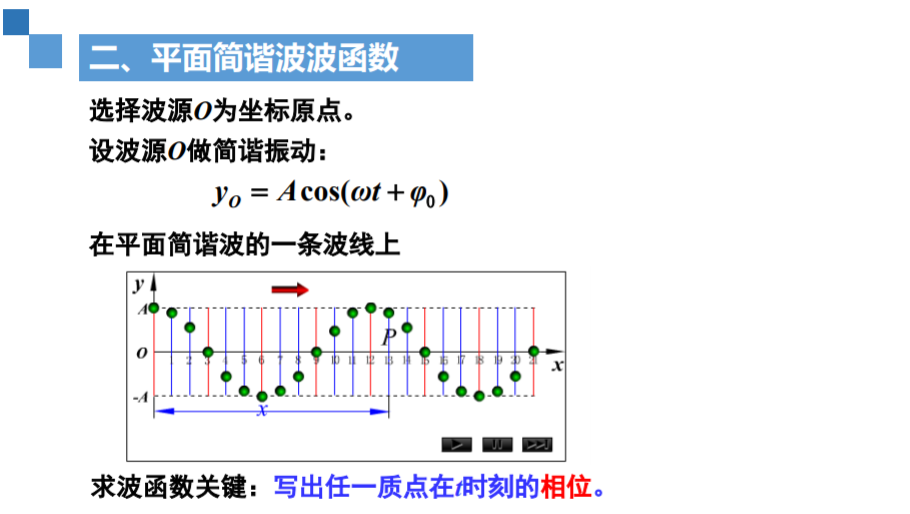
\includegraphics[width=13cm, height=8cm]{D:/UniversityNote/PhyNote/10/1001.png}
    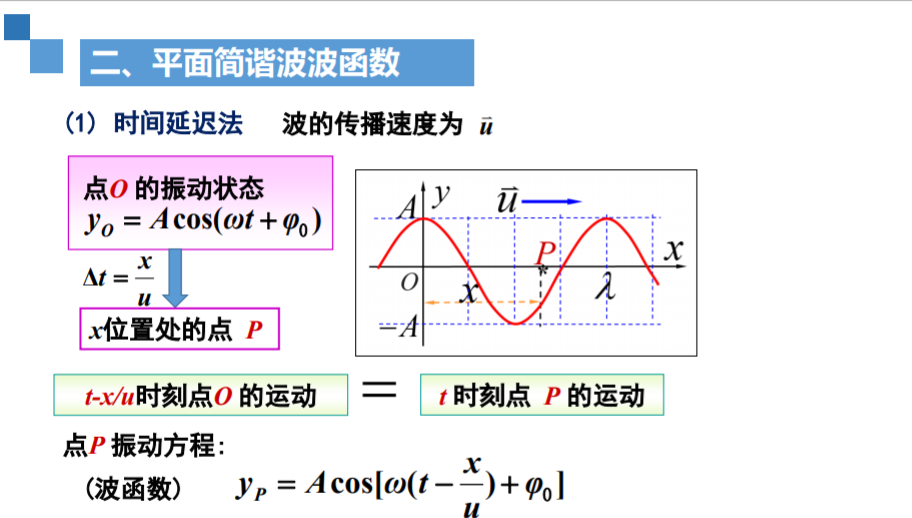
\includegraphics[width=13cm, height=8cm]{D:/UniversityNote/PhyNote/10/1002.png}
    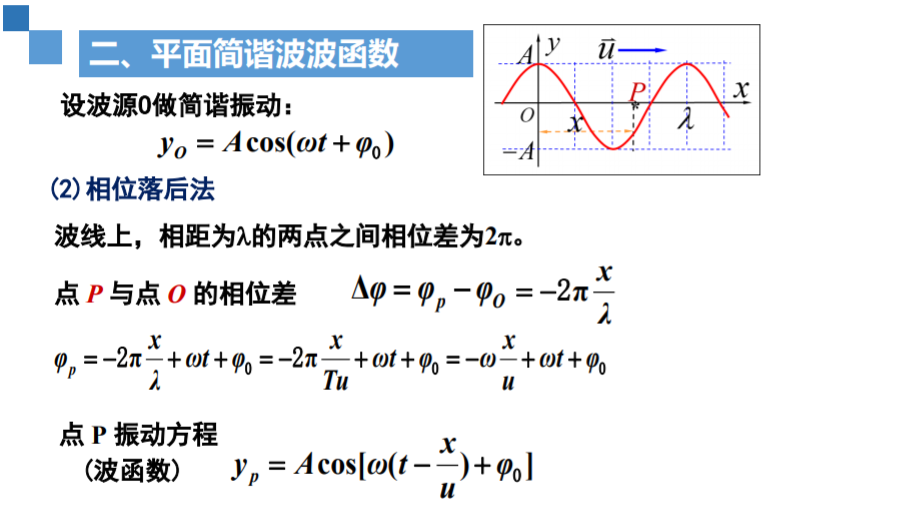
\includegraphics[width=13cm, height=8cm]{D:/UniversityNote/PhyNote/10/1003.png}
    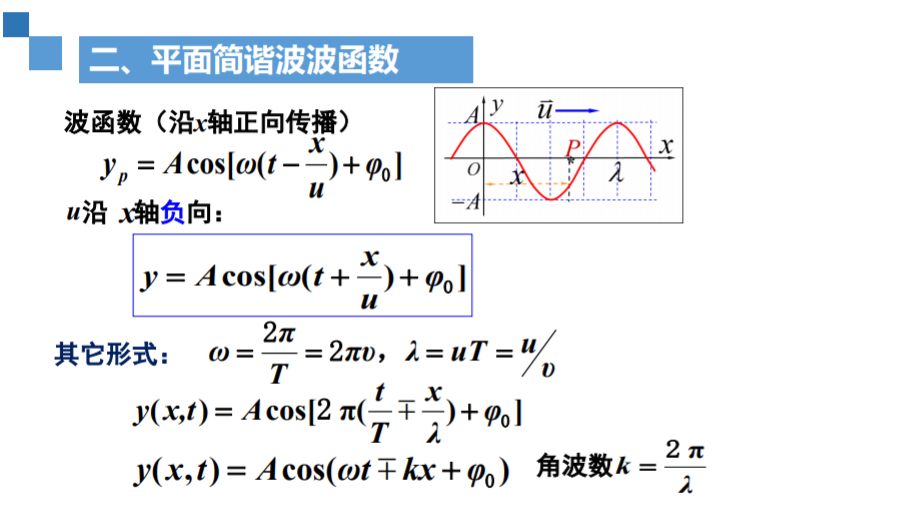
\includegraphics[width=13cm, height=8cm]{D:/UniversityNote/PhyNote/10/1004.png}
    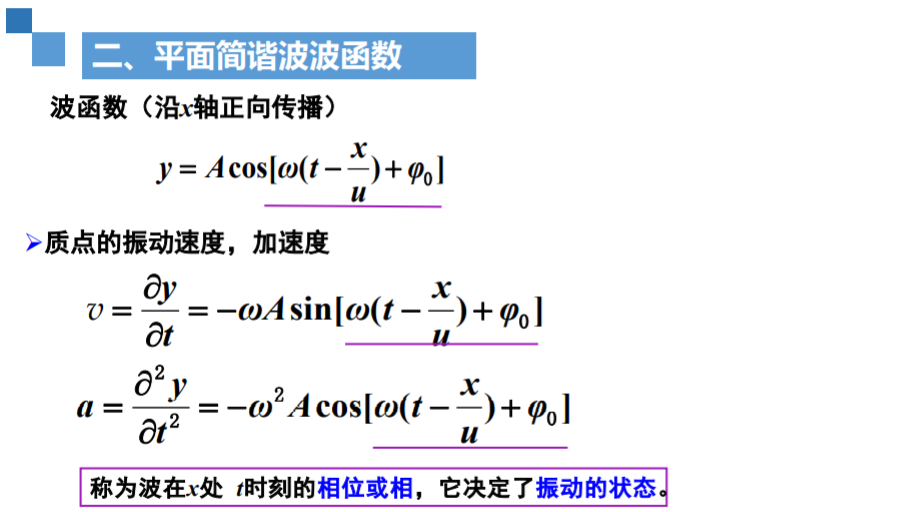
\includegraphics[width=13cm, height=8cm]{D:/UniversityNote/PhyNote/10/1005.png}

    波函数(沿x轴正向传播):$y = Acos[\omega(t - \frac{x}{u}) + \phi_0]$

    对于某一给定的相位
    \[\omega (t - \frac{x}{u}) = \mbox{常量}\phi\]

    两边对t求导可得相位的传播速度
    \[\frac{dx}{dt} = u\]

    说明波的相位的传播速度就是波的速度u,所以波速u也称为相速度,它可以超过光速

\subsection{波函数的物理意义和波动方程}

    一、波函数的物理意义
    \[y = Acos[\omega(t - \frac{x}{u} + \phi_0)] = Acos[2\pi(\frac{t}{T} - \frac{x}{\lambda}) + \phi_0]\]

    1.x固定时,表示该点的振动方程,体现波的时间周期性

    2.当t一定时,表示该时刻波线上各点相对其平衡位置的位移,体现波的空间周期性

    3.若x、t均变化,表示波形沿传播方向的运动情况(行波)

    二、波动方程
    \[y = Acos[\omega(t - \frac{x}{u} + \phi_0)]\]

    对变量二次求导
    \[\frac{\partial^2y}{\partial t^2} = -\omega^2Acos[\omega(t - \frac{x}{u} + \phi_0)]\]
    \[\frac{\partial^2y}{\partial x^2} = -\frac{\omega^2}{u^2}Acos[\omega(t - \frac{x}{u} + \phi_0)]\]

    波动微分方程
    \[\frac{\partial^2y}{\partial x^2} = \frac{1}{u^2}\frac{\partial^2y}{\partial t^2}\]

    具有普适性,即对任意一维平面波都成立

\subsection{机械波的能量}

    一、波动能量的传播


\end{document}